\chapter{Probabilistic Localization}

% Nice source for non-overly technical descriptions of probabilty terms:
% http://www.stats.gla.ac.uk/steps/


\section{Introduction}
In previous chapters we assumed that the we had access to accurate
information about the state of the world.  For example, in Chapter
\ref{chap:pid} we developed a closed-loop controller for moving a
robot to a goal by repeatedly comparing the robot's current location
to the goal location.  This raises the question of how we can know the
exact location of the robot.  The short answer is that we can't.  It
is possible to estimate the robot's location by using two general
sources of information:

\begin{itemize}
\item \textbf{Sensors} - There are a wide range of sensors that can
  provide information about the position of a robot.  Cameras may be
  used to detect landmarks.  Depth sensors may be used to estimate the
  robot's position in a map.  Bump sensors may be used to determine
  when the robot is in contact with an obstacle.
  
\item \textbf{Dead reckoning} - Assuming the initial location of a robot is
  known, it's location at some later time can be estimated by
  considering the control signals that have been applied.  If we send
  commands telling the robot to move forward at 1m/s for 1s, the robot
  should end up one meter ahead of the initial location.
\end{itemize}

There is inherent uncertainty associated with each of these sources of
information. No sensor is perfect. Dead reckoning is never perfectly
reliable. The goal of this chapter is to introduce a probabilistic
framework that will make it possible to represent and reason about
this uncertainty.

%Two goals for this chapter: introduce probabilistic representations and 
%addresss localization one of the key problems in robotics. 



For the sake of concreteness, this chapter will focus on probabilistic
representations of a robot's location, but the same mathematical tools
are useful for representing any uncertain information.



\section{Discrete Probability Distributions}

A \vocab{discrete random variable}, usually expressed as an upper-case
letter such as $X$, is a variable that can take on a fixed number of
possible values.  A \vocab{probability distribution}, also called a
\vocab{probability mass function}, is a function that maps from each
possible value of the random variable to its probability.

As a simple example, consider a Boolean random variable $H$ that
describes the possible outcomes of flipping a coin.  In this case, the
possible values for $H$ are $True$ indicating that the coin landed on
heads or $False$ indicating that the coin landed on tails.  The
probability mass function for a fair coin is then
\begin{align*}
P(H=True) = .5\\
P(H=False) = .5
\end{align*}

In the case of Boolean variables we often use the
more concise convention of indicating an assignment of true using a
lower case variable, so that $P(H=True)$ could be expressed as $P(h)$
and $P(H=False)$ could be expressed as $P(\neg h)$.

A valid probability mass function must satisfy the following
conditions:

\begin{itemize}
\item Probabilities must not be negative or greater than one:
  \[0 \leq P(X = {x_i}) \leq 1 \text{ for all } x_i\]
\item The probability mass function must sum to one:
  \[\sum_{x_i} P(X = {x_i}) = 1\]
\end{itemize}

Discrete random variables need not be Boolean-valued.  In particular,
a random variable may be used to describe our uncertainty about the
location of a robot, with each possible robot location corresponding
to a value for the random variable, and the probability distribution
describing our beliefs about which location is correct. For example,
consider the problem of tracking the location of a robot in a
one-dimensional world (perhaps our autonomous locomotive from Chapter
\ref{chap:pid}).  Figure \ref{fig:histograms} illustrates the idea.
The horizontal location of each bar corresponds to a discretized value
for the position variable, while the height of the bars correspond to
the value of the probability mass function for that position. Notice
that the height of all bars must always sum to one, since we know that
the robot must be located at some location.  The same information may
also be presented in tabular form as illustrated in Figure
\ref{fig:prob-tables}.

\begin{figure}
  \begin{center}
    \begin{subfigure}[b]{0.3\textwidth}
      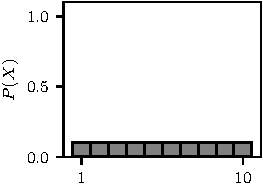
\includegraphics[]{probability/figs/uniform_hist.pdf}
      \caption{}
    \end{subfigure}
    \begin{subfigure}[b]{0.3\textwidth}
      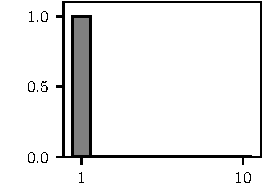
\includegraphics[]{probability/figs/certain_hist.pdf}
      \caption{}
    \end{subfigure}
    \begin{subfigure}[b]{0.3\textwidth}
      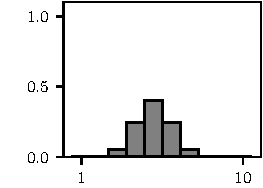
\includegraphics[]{probability/figs/gauss_hist.pdf}
      \caption{}
    \end{subfigure}
  \end{center}
  \caption{Sample histogram probability distributions describing our
    belief about the location of a robot in a one-dimensional
    environment. (a) Uniform distribution representing a complete lack
    of knowledge about the location of the robot. (b) Certain
    knowledge that the robot is in location 1. (c) Belief that the
    robot is most likely to be in location 5, but may be in nearby
    locations to the left or right.}
  \label{fig:histograms}
\end{figure}


\begin{figure}
  \begin{center}
    \begin{subfigure}[b]{0.3\textwidth}
       \begin{center}
      \begin{tabular}[b]{|l|l|}
    \hline
    X            & P(X) \\
    \hline
    1       & .1    \\
    \hline
    2        & .1   \\
    \hline
    3        & .1     \\
    \hline
    4        & .1      \\
    \hline
    5   & .1     \\
    \hline
    6      & .1   \\
    \hline
    7   & .1  \\
    \hline
    8      & .1     \\
    \hline
    9 & .1    \\
    \hline
    10 & .1    \\
    \hline
      \end{tabular}
       \end{center}
      \caption{}
    \end{subfigure}
    \begin{subfigure}[b]{0.3\textwidth}
       \begin{center}
        \begin{tabular}[b]{|l|l|}
     \hline
    X            & P(X) \\
    \hline
    1       & 1.0    \\
    \hline
    2        & 0   \\
    \hline
    3        & 0     \\
    \hline
    4        & 0      \\
    \hline
    5   & 0     \\
    \hline
    6      & 0   \\
    \hline
    7   & 0  \\
    \hline
    8      & 0     \\
    \hline
    9 & 0    \\
    \hline
    10 & 0    \\
    \hline
        \end{tabular}
         \end{center}
      \caption{}
    \end{subfigure}
    \begin{subfigure}[b]{0.3\textwidth}
      \begin{center}
        \begin{tabular}[b]{|l|l|}
    \hline
    X            & P(X) \\
    \hline
    1       & 0    \\
    \hline
    2        & .004   \\
    \hline
    3        & .054   \\
    \hline
    4        & .242     \\
    \hline
    5   & .400    \\
    \hline
    6      & .242   \\
    \hline
    7   & .054  \\
    \hline
    8      & .004     \\
    \hline
    9 & 0    \\
    \hline
    10 & 0    \\
    \hline
  \end{tabular} 
      \end{center}
      \caption{}
    \end{subfigure}
  \end{center}
  \caption{Tabular representations of the probability distributions
    illustrated in Figure \ref{fig:histograms}. Notice that the rows
    sum to one in each table.}
  \label{fig:prob-tables}
\end{figure}

In a more realistic scenario, the values for our random variable could
be entries in a grid corresponding to possible locations in a
two-dimensional workspace.  This idea is illustrated in Figure
\ref{fig:2dhist}.


\begin{figure}
  \begin{center}
  
      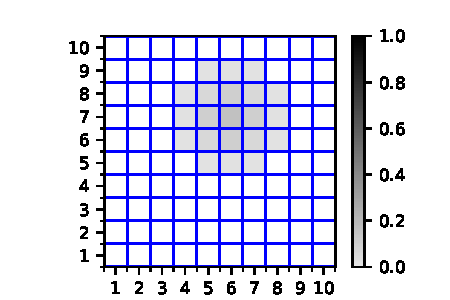
\includegraphics[]{probability/figs/2dhist.pdf}
   
  \end{center}
  \caption{Sample two-dimensional probability distribution.  In this
    example, shading is used to indicate the probability of the robot
    being located in a particular grid cell.}
  \label{fig:2dhist}
\end{figure}


%% \subsection*{Stop and Think}

%% \begin{exercise}
%%   How many random variables are illustrated in the following figure?
%% \end{exercise}



%% \begin{exercise}
%% Which of the following represent valid probability mass functions?
%% \end{exercise}



\subsection{Joint Probabilities}

Probabilistic models of complex systems generally involve multiple,
interacting, random variables.  The multivariate generalization of the
probability distribution is the \vocab{joint probability
  distribution}.  A joint probability distribution maps from every
possible outcome of all variables to the probability for that set of
assignments.  For example, In the case of our 1-d robot above, we can
introduce a second random variable representing the output of a wall
detection sensor that is designed to tell us when we are near one of
the two boundaries of the hallway (state 1 or state 10). This is
activated with probability .8 when the robot is at either end of the
hallway, .1 when it is one step away from either end and 0 for all
other locations.

In the case where we know nothing about the location of the robot, our
joint probability distribution will look like the following for our
location/sensor scenario:

\begin{table}[h!]
\begin{center}
 \begin{tabular}[b]{|l|l|l|}
    \hline
    X  & Z           & P(X,Z) \\
    \hline
    1  & $beep$      & .08    \\
    \hline
    1  & $\neg beep$ & .02    \\
    \hline
    2  & $beep$      & .01   \\
    \hline
    2  & $\neg beep$ & .09   \\
    \hline
    3  & $beep$      & 0      \\
    \hline
    3  & $\neg beep$ & .1     \\
    \hline
    \multicolumn{3}{|c|}{\ldots}   \\
    \hline
    8  & $beep$      & 0      \\
    \hline
    8  & $\neg beep$ & .1     \\
    \hline
    9  & $beep$      & .01   \\
    \hline
    9  & $\neg beep$ & .09   \\
    \hline
    10 & $beep$      & .08     \\
    \hline
    10 & $\neg beep$ & .02    \\
    \hline
 \end{tabular}
\end{center}
\caption{Joint probability distribution for robot position $X$ and wall sensor output $Z$.}
\label{tab:joint}
\end{table}

\subsubsection{Marginalization}

Given the full joint distribution we can always recover the probability
distribution for an individual variable through \vocab{marginalization}, or
summing out. In the general case, this can be expressed as:

\begin{equation} \label{eq:marginalization}
  P(A = a) = \sum_{b \in B} P(A = a,\; b)
\end{equation}

This means that if we want to calculate the probability of some
assignment to $A$ using the joint distribution, we just need to sum up
all of the rows in the table that match that assignment to $A$. For
example, given our location/sensor example above, we can recover the
probability that the robot is at position 2 as follows:

\[
\begin{split}
  P(X=2) & = P(X=2,\; beep) +  P(X=2,\; \lnot beep) \\
  & = .01 + .09 \\
  & = .1 
  \end{split}
\]

\subsection*{Stop and Think}

\begin{exercise}
Based on the joint probability distribution in Table \ref{tab:joint}, what is
$P(beep)$? What is $P(\lnot beep)$?
\end{exercise}


\subsubsection{Independence}
\label{sec:independence}
Two random variables are defined to be \vocab{independent} if and
only if
\begin{equation}
  P(A \cap B) = P(A)P(B).
\end{equation}
Intuitively, $A$ and $B$ are independent if knowing the value of $A$
 provides no information about the value of $B$.  For example,
whether or not a region will experience an earthquake on a particular
day is independent of the occurrence of a tornado: there is no reason
to believe that one will make the other more or less likely.  On the
other hand, whether a region will experience an earthquake on a given
day is \emph{not} independent of the possibility of a tsunami:
earthquakes can cause tsunamis, so knowing that one has occurred
increases the probability of the other.

The notion of independence is important for probabilistic
reasoning. In the example from the previous section, we saw a joint
probability distribution with two random variables.  In general,
applications involving probabilistic reasoning may involve \emph{many}
random variables. For example, consider a robot navigating through an
office building with 20 doors that may each be open or closed.
Assuming that the robot is unable to open doors, path planning in this
environment will require reasoning about the possible states of all
doors. In order to write down the full joint probability distribution
describing every possible combination of closed and open doors, we
would need a table with $2^{20}\approx 1,000,000$ rows. It is much
more efficient, in terms of both space and computation, to make the
assumption that the state of each door is independent of the state of
every other door. In that case we only need to store 20 individual
probability distributions with two rows each.  We can then reconstruct
the probability of any combination of closed and open doors by simply
multiplying together the appropriate 20 probabilities.

Note that \vocab{independence assumptions} of this sort may be useful
even if they aren't entirely correct.  In a real office building it is
unlikely that the states of individual doors will be entirely
independent. If the doorway to a suite of offices is open, there is
probably someone working in that suite, which would make it more
likely that the individual office doors will be open as well. This is
a case where it is necessary to settle for an approximately correct
answer in the interest of computational tractability.


\subsection*{Stop and Think}

\begin{exercise}
The probability that it will rain today, $P(R)$ is independent of the
probability of an earthquake, $P(E)$. Assuming $P(r) = .7$ and $P(e) =
.001$, what is the probability that it will be a rainy day with no
earthquake? $P(r, \lnot e) = ??$
\end{exercise}


\subsection{Conditional Probabilities}

Probability distributions like $P(X)$ are sometimes described as
\vocab{prior probabilities} because they describe our initial belief
about $X$ before we have taken any evidence into
account. \vocab{Conditional probabilities} allow us to express the
probability for one random variable, given that we know the value of
some other random variable.  Conditional probability is defined as
follows:

\begin{equation} \label{eq:conditional}
  P(A \mid B) = \frac{P(A \cap B)}{P(B)}
\end{equation}

Conditional probabilities provide a useful way of thinking about the
relationship between a robot's state and sensor data.  For robot
localization, some variables represent unknown state information that
we are attempting to estimate.  This unknown state information is
commonly denoted $X$.  On the other hand, some variables represent
\emph{known} values received from a sensor.  These values are commonly
denoted $Z$. For the purpose of localization, it would be useful to
have access to the conditional probability distribution $P(X \mid Z)$.
This is exactly the distribution over $X$ given our known sensor value
$Z$.

As an example of conditional probability, consider the case of a cliff
detection sensor designed to prevent a home-vacuuming robot from
falling down stairways.  In this case, $S$ is a Boolean random
variable indicating whether a stairway is actually present,
and the variable $Z$ is true if the cliff-detection sensor has
activated. The following table describes the full joint probability
distribution:


\begin{table}[h!]
  \begin{center}
    \begin{tabular}[b]{|l|l|l|}
      \hline
      $S$  & $Z$          & $P(S, Z)$ \\
      \hline
      T  & T & .0495    \\
      \hline
      T  & F & .0005    \\
      \hline
      F  & T & .095   \\
      \hline
      F  & F & .855   \\
      \hline
    \end{tabular}
  \end{center}
\end{table}

Using this table, along with Equations \ref{eq:marginalization} and
\ref{eq:conditional}, we can calculate, for example, the false
positive rate of our sensor: $P(Z = True \mid S = False)$.  In other words,
what is the probability that the sensor will indicate that a stairway
is present when it is not.

\[
\begin{split}
  P(Z = True \mid S= False) &= \frac{P(Z = True \cap S = False)}{P(S = False)} && \\
  & =  \frac{.095}{P(S = False)}&& \text{(From the third row of the table above)} \\
  & =  \frac{.095}{P(S = False, Z = True) + P(S = False, Z = False)}&&\text{(Marginalization)} \\
  & =  \frac{.095}{.095 + .855} = .1 &&
\end{split}
\]

\subsection*{Stop and Think}

\begin{exercise}
  Look back at table \ref{tab:joint}.  Apply definition \ref{eq:conditional} to calculate $P(X=0 \mid Z=beep)$.
\end{exercise}



\subsubsection{Conditional Independence}
Section \ref{sec:independence} introduced the idea of independent
random variables.  Now that we have an understanding of conditional
distributions we can introduce a second notion of independence that is
also a valuable tool in probabilistic reasoning.

\vocab{Conditional independence} is defined as follows:

A random variable $A$ is conditionally independent of $C$ given $B$
if and only if
\begin{equation}
  P(A \mid B, C) = P(A \mid B).
\end{equation}

Intuitively, this means that, if we already know $B$, then learning
something about $C$ doesn't tell us anything additional about
$A$. This is a bit more subtle than the definition of independence
introduced earlier. Stating that $A$ is conditionally independent from
$C$ given $B$ is not the same as saying that any two of those
variables are independent. As an example, consider the following scenario:
\begin{itemize}
\item $A$: The east door to the mall is locked
\item $B$: The mall is open for business
\item $C$: The west door to the mall is locked
\end{itemize}
In this case, $A$ and $C$ are not independent.  If I learn that one
door is locked, that increases my belief that the other will be
locked as well. However, they \emph{are} conditionally independent
given $B$: if I already know whether or not the mall is open, then
learning the state of the west door doesn't give me any additional
information about east door.



\subsection{Bayes' Rule}

Unfortunately definition (\ref{eq:conditional}) often isn't useful
for determining $P(X \mid Z)$ because it requires us to have access to
the full joint probability distribution $P(X, Z)$.  In practice, that
full distribution is usually not easy to obtain in an explicit form.
\vocab{Bayes' rule} or \vocab{Bayes' theorem} is tremendously useful
here.  Baye's rule can be expressed as follows:

\begin{equation}
  P(X \mid Z) =  \frac{P(Z \mid X) P(X)}{P(Z)}
\end{equation}

Bayes' rule provides a recipe for taking the prior probability $P(X)$
that describes our initial beliefs about the robot's state and
calculating a \vocab{posterior probability} $P(X \mid Z)$ that
describes our updated belief after into account information from a
sensor reading.

In order to apply Bayes' rule, we need to know two things:

\begin{itemize}
  \item $P(Z \mid X)$ - The conditional probability of sensor readings
    given state information.  This is often described as the
    \vocab{sensor model}. It simply captures what we know about
    how our sensor works.
    \item $P(X)$ - The prior distribution over our state variable. 
\end{itemize}
It turns out we don't need to know $P(Z)$ explicitly.  It can be
calculated from $P(Z \mid X)$ and $P(X)$ using the \vocab{total
  probability formula}:
\begin{equation}\label{eq:total}
  P(Z) = \sum_{x \in X} P(Z \mid X=x) P(X=x)
\end{equation}


Alternatively, it is common to to replace $P(Z)$ using a
\vocab{normalizing constant} $\alpha$ defined as
\[\alpha = \frac{1}{P(Z)}.\] This results in the following alternate form of Bayes' rule:
\begin{equation}
  P(X \mid Z) = \alpha P(Z \mid X) P(X)
\end{equation}
This formulation takes advantage of the fact that we know that $P(Z)$
is the same for every state. We can simply solve for the value of
$\alpha$ that makes the posterior probability sum to one.

\subsubsection{Bayes' Rule Example}

Consider another one-dimensional robot that may be in
one of ten discrete locations.  In this case, there is a radio beacon
located at location \textbf{5} and the robot has a sensor that detects
the beacon with a probability that is related to distance.  The
scenario is illustrated in Figure \ref{fig:robot_radio}.

\begin{figure}
    \begin{center}
  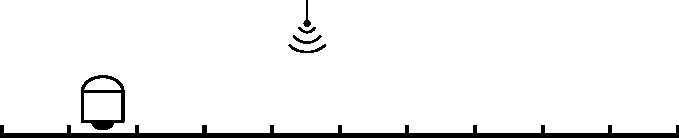
\includegraphics[]{probability/figs/robot_radio.pdf}
   \end{center}
  \caption{A scenario with ten discrete robot locations.  There is a
    radio beacon at location 5.}
  \label{fig:robot_radio}
\end{figure}


When the robot is in the same location as the beacon, it will be
detected with a probability of 1. When the robot is one step away, it
will be detected with a probability of .5. The probability of detection
continues to drop off at a rate of 50\% for each step away from the
beacon. Figure \ref{fig:radio_sensor} illustrates this sensor model.

\begin{figure}
    \begin{center}
  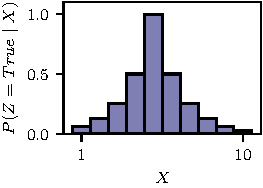
\includegraphics[]{probability/figs/sensor_true.pdf}
   \end{center}
  \caption{Sensor model for our radio beacon detector.  The probability
    that the sensor will activate falls off as the robot moves further
    away from the beacon. Notice that this figure is \emph{not}
    illustrating a probability distribution of the type shown in
    Figure \ref{fig:histograms}. In this case the probabilities
    don't need to sum to one.}
  \label{fig:radio_sensor}
\end{figure}


In this scenario, Bayes' rule allows us to update our belief about
where the robot is located based on the signal received from the radio
sensor. Let's assume that our prior probability distribution over the
robot's location looks like this:
\begin{center}
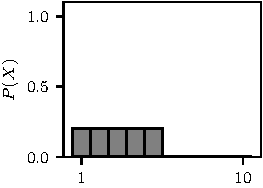
\includegraphics[]{probability/figs/left_hist.pdf}
\end{center}
This prior distribution $P(X)$ reflects that robot is equally likely
to be in any of the five locations on the left, with a .2 probability
of being in each.

Now assume that the robot takes a reading from its beacon-detector and the
value is $True$. Figure \ref{fig:bayes} illustrates the steps of
applying Bayes' rule to calculate the posterior distribution.  First,
the prior probability associated with each state $P(x_i)$ is
multiplied by the value of the sensor model at that state $P(Z = True
\mid X = x_i)$.  The resulting values are then re-scaled to sum to one.

\begin{figure}
  \begin{center}
    \begin{subfigure}[b]{0.3\textwidth}
      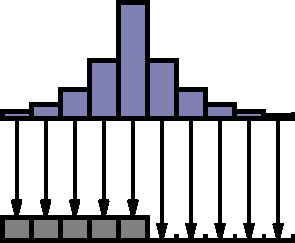
\includegraphics[width=1.5in]{probability/figs/Bayes1.pdf}
      \caption{ }
    \end{subfigure}
    \begin{subfigure}[b]{0.3\textwidth}
      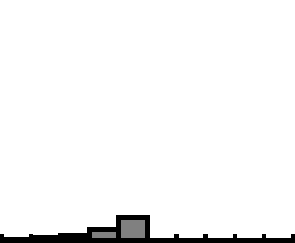
\includegraphics[width=1.5in]{probability/figs/Bayes2.pdf}
      \caption{}
    \end{subfigure}
    \begin{subfigure}[b]{0.3\textwidth}
      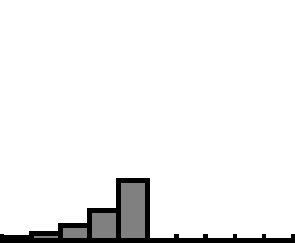
\includegraphics[width=1.5in]{probability/figs/Bayes3.pdf}
      \caption{}
    \end{subfigure}
  \end{center}
  \caption{Using Bayes' rule to update state estimates based on a
    sensor reading. (a) The bar graph on the top represents the sensor
    model $P(Z=True \mid X)$.  The bar chart on the bottom represents
    the prior distribution over the robot's location $P(x)$ The
    vertical arrows represent multiplication: the value of the sensor
    model at each state is multiplied by the prior probability for the
    corresponding state. (b) The resulting products. Note that these
    values do \emph{not} sum to one.  (c) The values at each state
    re-scaled (or \vocab{normalized}) to make the total sum to 1. The
    result is the posterior probability distribution $P(X \mid Z)$}
  \label{fig:bayes}
\end{figure}

Let's do a detailed run-through through of the example in Figure
\ref{fig:bayes} to see how the steps follow from the
application of Bayes' rule. Bayes' rule may be used to calculate the
posterior probability that the robot is in any particular state.  For
example, calculating the posterior for state 1 looks like the
following:
\[ P(X=1 \mid Z=True) = \alpha P(Z=True \mid X=1) P(X=1) \]
Substituting  $P(Z=True \mid X=1) = 0.0625$ from the sensor model and  $P(X=1) = .2$ from the prior distribution yields:
\[ P(X=1 \mid Z=True) = \alpha ( 0.0625 \times .2) = 0.0125\alpha   \]
This calculation is repeated for all values of $X$:
\begin{alignat*}{3}
P(X=1 \mid Z=True) &=\alpha ( 0.0625 \times .2) ~&=&~ 0.0125\alpha   \\
P(X=2 \mid Z=True) &=\alpha ( 0.0125 \times .2) ~&=&~ 0.025\alpha   \\
P(X=3 \mid Z=True) &=\alpha ( 0.25 \times .2) ~&=&~ 0.05\alpha   \\
P(X=4 \mid Z=True) &=\alpha ( 0.5 \times .2) ~&=&~ 0.1\alpha   \\
P(X=5 \mid Z=True) &=\alpha ( 1.0 \times .2) ~&=&~ 0.2\alpha   \\
P(X=6 \mid Z=True) &=\alpha ( 0.5 \times 0) ~&=&~ 0   \\
&...&& \\
\end{alignat*}
All that remains is to determine $\alpha$ by solving for the value
that makes the total probability sum to 1:
\[0.0125\alpha +  0.025\alpha + 0.05\alpha  + 0.1\alpha + 0.2\alpha  = 1.0\]
\[\alpha \approx 2.581\]
Substituting 2.581 for $\alpha$ gives us the final posterior probability distribution across states:
\begin{alignat*}{3}
P(X=1 \mid Z=True) &= 0.0125\alpha  ~&\approx&~ 0.0323   \\
P(X=2 \mid Z=True) &= 0.025\alpha  ~&\approx&~ 0.0645   \\
P(X=3 \mid Z=True) &= 0.05\alpha  ~&\approx&~ 0.1290   \\
P(X=4 \mid Z=True) &= 0.1\alpha ~&\approx&~ 0.2581  \\
P(X=5 \mid Z=True) &= 0.2\alpha ~&\approx&~ 0.5161\   \\
P(X=6 \mid Z=True) &=0 &&   \\
&...&& \\
\end{alignat*}


\section{Recursive State Estimation}
\label{sec:recursive_estimation}


We now have the tools to formalize the central computational problem
raised in this Chapter.  The fundamental goal in robot localization is
to estimate a robot's position based on the full history of sensor
readings and actions taken by the robot.  This can be expressed as
follows:
\begin{equation}\label{eq:localization_prob}
  Bel(X_t) = P(X_t | U_0, Z_0,\; U_1, Z_1,\; ...,\;U_{t}, Z_{t})
\end{equation}
where the subscripts indicate discrete time intervals and the $U$
variables represent the action choices made by the robot at each time
step.  According to this definition, the \vocab{belief state} $Bel(X_t)$ is
defined to be conditional distribution over the robot's location at
time step $t$ given full history of actions and sensor readings leading up
to time $t$.

We are already halfway to the solution. At the beginning of this
Chapter we claimed that keeping track of a robot's location involves
two sources of information: sensor data and dead reckoning. As we've
seen above, Bayes' rule exactly solves the problem of incorporating
sensor data to update our beliefs about the robot's location.

In order to incorporate dead reckoning we need a probabilistic model of
how the robot's actions impact its state.  This can be expressed with
the following conditional probability distribution:
\[P(X_t \mid X_{t-1}, U_{t})\]
This distribution is often described as the \vocab{motion model} for
the robot. Notice that this formulation involves an implicit
conditional independence assumption in that the state distribution at
time step $t$ only depends on the most recent state and
action. Expressed formally, we are assuming that:
\begin{equation}
  P(X_t \mid X_{t-1}, U_{t}) = P(X_t \mid X_{t-1}, U_{t}, X_{t-2}, U_{t-1},..., X_0, U_1)
\end{equation}
This is called the \vocab{Markov assumption}.  This assumption may be
expressed in English as ``The future is independent of the past given
the present.''

The Markov assumption is key to developing a tractable algorithm for
tracking the belief state.  At first glance, the formulation of the
localization problem in Equation \ref{eq:localization_prob} should be
worrying. The history of sensor readings and action choices will
continue to grow without bound over time.  This raises the concern
that the computational cost of maintaining our belief state will also
continue to grow as we accumulate more and more history that needs to
taken into account.  The Markov assumption provides a way out of that
dilemma.

The full \vocab{recursive state estimation} algorithm can be expressed
as follows:

\begin{align}
  &Bel^{-}(X_t) = \sum_{x_i \in X_{t-1}} P(X_t \mid X_{t-1} = x_i,\; U_{t}) Bel(X_{t-1}=x_i) & \text{(Prediction)}\\
  &Bel(X_t) = \alpha P(Z_t \mid X_{t-1}) Bel^{-}(X_t) & \text{(Correction)}
\end{align}

In the \textbf{prediction} stage, we update the belief state based on
the robot's latest action by applying the total probability theorem
(Equation \ref{eq:total}) to the motion model to sum across all
possible values for the previous state.  The ${}^-$ superscript
indicates that the result is the estimated belief state before
information about any sensor readings has been incorporated.  This is
referred to as the ``prediction'' step because we are predicting where
the robot is likely to end up based on the action it selected.


In the \textbf{correction} stage we apply Bayes' rule to update the
belief state based on the latest sensor reading, exactly as was
discussed in the previous section. This is referred to as the
``correction'' step because we are revising our prediction by
incorporating the latest sensor information.

These two stages alternate indefinitely, with the belief state
calculated at each time step serving as the prior belief state for the
next time step.  Assuming that the Markov assumption is correct, and
that the motion and sensor models are accurate, this algorithm
correctly tracks the probability distribution over the robot's
location over time.

One thing to keep in mind is that a perfect localization algorithm
doesn't give us perfect information about the location of the
robot. Our knowledge of the robot's location is fundamentally limited
by the uncertainty in our sensor model, the uncertainty in our motion
model, and our uncertainty about the robot's initial location when
localization began.  What we can guarantee is that the recursive state
estimation algorithm above gives the best possible estimate given
these various sources of uncertainty.


\subsubsection{Prediction Example}


Figure \ref{fig:motion_update} illustrates the process of applying the
prediction formula. In the motion model for this example, there are
three possible outcomes when the robot attempts to move to the right:
There is a 60\% chance that the action works as expected and the robot
moves one cell to the right.  There is a 20\% chance that the action
fails and the robot stays in the same location, and there is a 20\%
chance that the robot overshoots and moves two positions to the right.

Figure \ref{fig:motion_update}(a) illustrates the calculation for just
state 5. Given this motion model, there are three possible ways the robot could
end up in state 5: it could start in state 3 and overshoot, it could
start in state 4 with the expected outcome, or it could start in state
5 and fail to move.  The prediction formula sums across these three
possibilities:

\begin{align*}
  Bel^{-}(X_t = 5) =& \sum_{x_i \in X_{t-1}} P(X_t = 5 \mid X_{t-1} = x_i,\; U_{t} = Right) Bel(X_{t-1}=x_i)\\
  =& P(X_t = 5 \mid X_{t-1} = 3,\; U_{t} = Right) Bel(X_{t-1}=3)\; +\\
  &P(X_t = 5 \mid X_{t-1} = 4,\; U_{t} = Right) Bel(X_{t-1}=4)\; +\\
  &P(X_t = 5 \mid X_{t-1} = 5,\; U_{t} = Right) Bel(X_{t-1}=5)\\
  =& (.2 \times .25) + (.6 \times .5) + (.2 \times .25)\\
  =& .4
\end{align*}

The full belief prediction update involves repeating this calculation
for each state.  The result is illustrated in figure \ref{fig:motion_update}(b)

\begin{figure}
  \begin{center}
    \begin{subfigure}[b]{0.4\textwidth}
      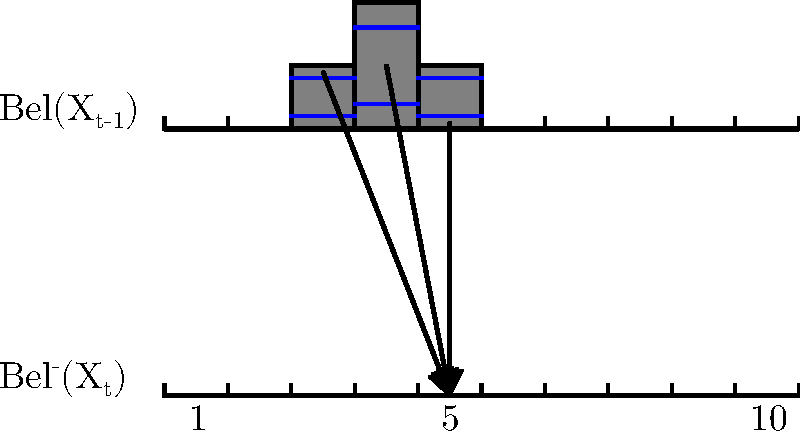
\includegraphics[height=1.5in]{probability/figs/motion_calc.pdf}
      \caption{ }
    \end{subfigure} \hspace*{1in}
    \begin{subfigure}[b]{0.4\textwidth}
      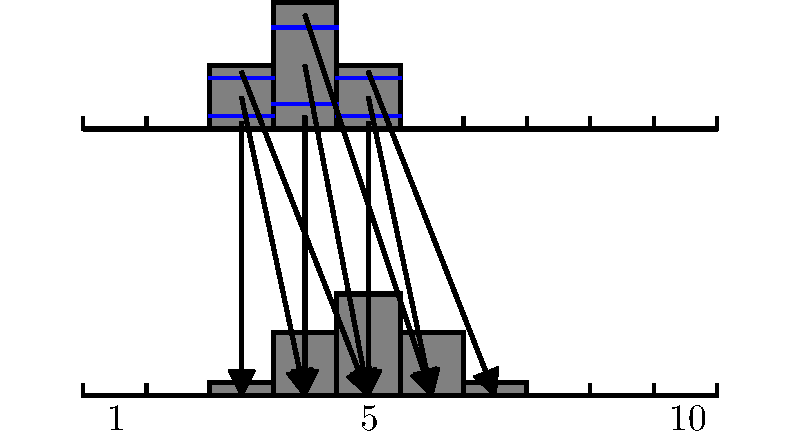
\includegraphics[height=1.5in]{probability/figs/motion_calc_done.pdf}
      \caption{}
    \end{subfigure}
  \end{center}
  \caption{Using the prediction formula to update the belief state
    based on the motion model. (a) Each arrow represents a term in the
    sum for $Bel^{-}(X_t = 5)$.  (b) The final belief distribution
    after all sums have been calculated.}
  \label{fig:motion_update}
\end{figure}

\subsection{Efficiency Considerations}

The discrete, grid-based state representation assumed so far raises
some of the same efficiency issues that were discussed in Chapter
\ref{chap:planning}.  In particular, the space and
computational requirements grow exponentially with the dimensionality of
the robot's state.  Two-dimensional localization may be tractable, but
once we add orientation and three-dimensional location, the problem
quickly becomes un-manageable. There is also a trade-off between the
granularity of the discretization and the precision of localization.
Finer granularity may result in better localization, but only at the
expense of additional computational cost.

In practice, it is common to use one of two alternative formulations
of the recursive state estimation algorithm described above: the
\vocab{Kalman filter} or the \vocab{particle filter}.

\section{Kalman Filter}

The overall form of the Kalman filter algorithm is the same as the
recursive state estimation algorithm described above: There is a
prediction phase in which the state estimate is projected forward
through time, followed by a correction phase in which the state
estimate is updated according to the latest sensor reading. The
difference is that the Kalman filter uses an alternative
representation of the belief state, and makes some strong assumptions
about the form of the motion and sensor models:

\begin{itemize}
\item The belief state is represented as a multi-variate normal
  distribution.
\item The state update and sensor models must be linear.
\item The noise in both the motion and sensor models must be described
  by multi-variate normal distributions.
\end{itemize}

If these assumptions are satisfied, the Kalman filter provides an
efficient and optimal localization algorithm.

\subsection{Linear State Dynamics}

As an example, consider the following system of difference equations
that describe the motion of an object moving at a fixed velocity in
two dimensions:

$x_{t+1} = x_{t} + \dot{x}_t dt$ \\
$y_{t+1} = y_{t} + \dot{y}_t dt$ \\
$\dot{x}_{t+1} =  \dot{x}_t$ \\
$\dot{y}_{t+1} =  \dot{y}_t$ \\

In these equations $x_t$ and $y_t$ represent the x and y coordinates
of the object at time $t$, $\dot{x}_t$ and $\dot{x}_t$ represent the
instantaneous velocity, and $dt$ represents the time interval between
updates. The first two equations describe the motion of the object,
while the second two equations simply describe the fact that the
velocity remains constant over time.

This system can be described more concisely by representing the
state information as a vector, and the series of difference equations
as the matrix product:
\[
\textbf{x}_{t+1}  = \mathbf{F} \textbf{x}_t
\]

Where $\textbf{x}_t$ represents the state vector and $\mathbf{F}$ is a
matrix that describes the update equations:

$\displaystyle \textbf{x}_t =\begin{bmatrix}
 x_t \\
y_t \\
 \dot{x}_t\\
\dot{y}_t\\
\end{bmatrix}$, \hspace*{.2in}
$\displaystyle \mathbf{F} = 
 \begin{bmatrix}
 1 & 0 & dt & 0 \\
 0 & 1 & 0 & dt \\
 0 & 0 & 1 & 0 \\
 0 & 0 & 0 & 1 \\
\end{bmatrix}$

We may also want to represent the fact that there it is possible to
apply a control signal to the object.  For example, we could update
our update equations with terms representing an application of
force that impacts the objects velocity:

\newcommand{\highlighteq}[1]{%
  \colorbox{yellow!50}{$\displaystyle#1$}}

$x_{t+1} = x_{t} + \dot{x}_t dt$ \\
$y_{t+1} = y_{t} + \dot{y}_t dt$ \\
$\dot{x}_{t+1} =  \dot{x}_t + \highlighteq{\ddot{x}_t dt}$ \\
$\dot{y}_{t+1} =  \dot{y}_t + \highlighteq{\ddot{y}_t dt}$ \\

We can incorporate this control signal by adding an additional term to
our linear state update equation:

\[
\textbf{x}_{t+1}  = \mathbf{F} \textbf{x}_t + \mathbf{B} \textbf{u}_t
\]

where 

$\displaystyle \textbf{u}_t =\begin{bmatrix}
 \ddot{x}_t\\
 \ddot{y}_t\\
\end{bmatrix}$, \hspace*{.2in}
$\displaystyle \mathbf{F} = 
 \begin{bmatrix}
 0 & 0  \\
 0 & 0  \\
 dt & 0  \\
 0 & dt  \\
\end{bmatrix}$.

Finally, we need to take into account that the motion model should not
be completely deterministic.  We don't expect any model to make
perfect predictions in a real-world system.  The Kalman filter works
under the assumption that system noise is normally distributed. We can
incorporate noise by adding one final term to our state update equation:

\begin{equation}
  \mathbf{x}_t = \mathbf{F} \mathbf{x}_{t-1} + \mathbf{B} \mathbf{u}_{t-1} + \mathbf{w}_{t-1}
\end{equation}

Where $\mathbf{w}$ is a random vector drawn from a normal distribution with mean zero and covariance $Q$:

\[\mathbf{w} \sim \mathcal{N}(\mathbf{0},\mathbf{Q})\]


\subsection{Linear Sensor Model}

The sensor model for a Kalman filter is also represented by a linear
model corrupted with normally-distributed noise.  The sensor model has
the following form:

\begin{equation}
  \mathbf{z}_t = \mathbf{H} \mathbf{x}_t + \mathbf{v}_t
\end{equation}

Where $\mathbf{z}_t$ represents the observed sensor reading and 
$\mathbf{v}_t \sim \mathcal{N}(\mathbf{0},\mathbf{R})$ represents
normally distributed sensor noise with covariance $\mathbf{R}$.

Continuing the example from above, we will assume that we have access
to a sensor that provides estimates about the coordinates of the
object, but doesn't provide any direct information about the
velocity. In this case, we have

\[
\mathbf{H} = 
\begin{bmatrix}
  1& 0& 0& 0 \\
  0& 1& 0& 0
\end{bmatrix}
\]

\subsection{Kalman Filter Algorithm}

The Kalman filter stores the belief state as a normal distribution.
The mean of the distribution $\hat{\mathbf{x}}$ represents the current
best estimate of the system state, while the covariance $\mathbf{P}$
represents the amount (and shape) of the current uncertainty.  As with
the recursive state estimation algorithm described in Section
\ref{sec:recursive_estimation}, the algorithm proceeds in two stages:
a prediction stage, followed by a correction stage.  Again, the ${}^-$
superscript indicates that the result is the estimated belief state
before sensor readings have been incorporated.  The full algorithm is
outlined in Figure \ref{fig:kalman_algorithm}.


\begin{figure}
  \begin{framed}
    \textbf{Inputs}: Initial state estimate $\hat{\mathbf{x}}_0$ and covariance  $\mathbf{P}_0$.
    \vspace{1em}
    \begin{itemize}
      \item \textbf{Repeat forever:}
\begin{itemize} 
\item \textbf{Prediction}
  \begin{itemize}
    \item Project the state forward according to the motion model:
      \begin{equation}
        \label{eq:kal_update_x}
    \hat{\mathbf{x}}^-_t = F \hat{\mathbf{x}}_{t-1} + B \mathbf{u}_{t-1}
  \end{equation}
  \item Project the covariance of the state estimate forward: 
  \begin{equation}
        \label{eq:kal_update_P}
    \mathbf{P}^-_t = F \mathbf{P}_{t-1}F^T + \mathbf{Q}
  \end{equation}
  \end{itemize}
  
\item \textbf{Correction}
  \begin{itemize}
  \item Compute the Kalman gain:
    \begin{equation}
      \label{eq:kal_correct_K}
      \mathbf{K}_t = \mathbf{P}^-_t H^T(H \mathbf{P}^-_t H^T +  \mathbf{R})^{-1}
    \end{equation}
  \item Use the sensor reading to update the state estimate:
    \begin{equation}
      \label{eq:kal_correct_x}
      \hat{\mathbf{x}}_t =\hat{\mathbf{x}}^-_t + \mathbf{K}_t (\mathbf{z}_t - H \hat{\mathbf{x}}^-_t)
    \end{equation}
  \item Update the covariance of the state estimate:
    \begin{equation}
      \label{eq:kal_correct_P}
    \mathbf{P}_t =  \mathbf{P}^-_t - \mathbf{K}_t H\mathbf{P}^-_t\end{equation}
  \end{itemize}
\end{itemize}
\end{itemize}
\end{framed}

\caption{Kalman filter algorithm.}
  \label{fig:kalman_algorithm}
\end{figure}


\begin{figure}
  \begin{center}
    \begin{subfigure}[b]{0.4\textwidth}
      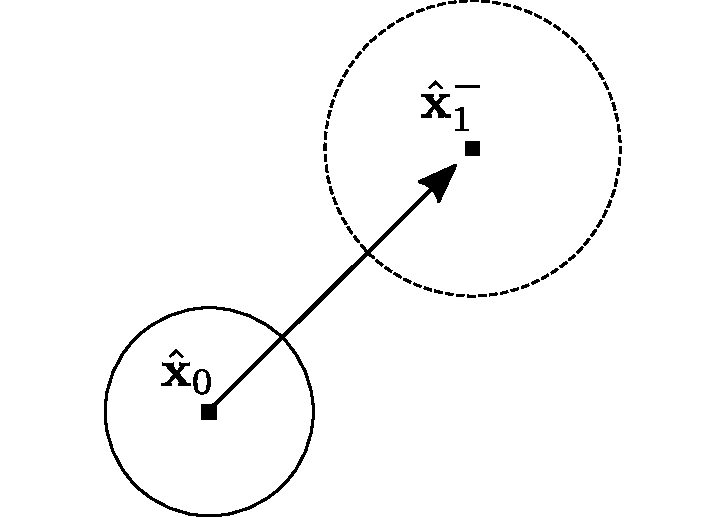
\includegraphics[height=1.5in]{probability/figs/kalman/kalman_pred.pdf}
      \caption{ }
    \end{subfigure} \hspace*{1in}
    \begin{subfigure}[b]{0.4\textwidth}
      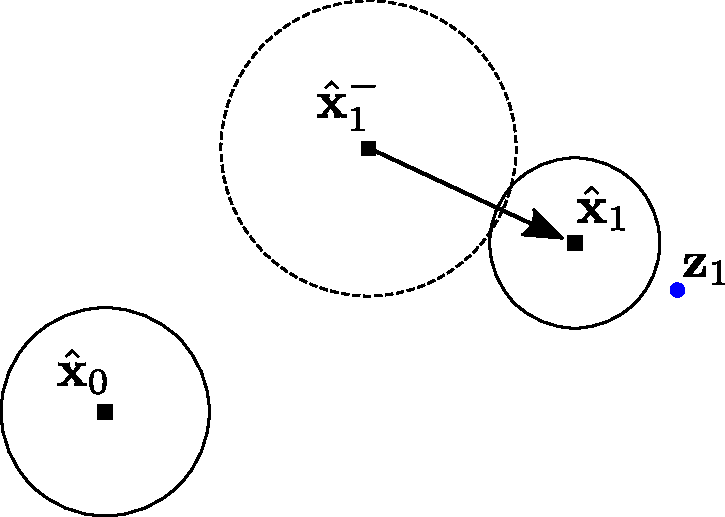
\includegraphics[height=1.5in]{probability/figs/kalman/kalman_correct.pdf}
      \caption{}
    \end{subfigure}
  \end{center}
  \caption{Kalman filter example. (a) \textbf{Prediction phase:}  The state
    estimate is updated according to the linear motion model.  The
    solid circle represents the initial uncertainty, while the dotted
    circle represents the increased uncertainty based on the known noise
    in the motion model.  (b) \textbf{Correction phase:}.  The state
    prediction is adjusted in the direction of the sensor reading.
    The uncertainty in the estimate decreases as a result of
    incorporating the sensor information.}
  \label{fig:kalman_demo}
\end{figure}

The prediction phase of the algorithm updates the state estimate
according to the motion model (Equation \ref{eq:kal_update_x}) and
increases the estimated uncertainty according the noise in the motion
model (Equation \ref{eq:kal_update_P}). This is illustrated in
\ref{fig:kalman_demo}.


The correction phase involves updating the state estimate to account
for the most recent sensor reading. Equation \ref{eq:kal_correct_x}
can be understood as taking a weighted average between the prediction
estimate and the estimate that is suggested by the latest sensor
value. The \vocab{Kalman gain}, calculated in Equation
\ref{eq:kal_correct_K}, represents the optimal trade-off between those
two sources of information. Intuitively, the Kalman filter places a
higher weight on the sensor when the sensor noise is low relative to
the uncertainty in the state estimate. Conversely, the Kalman filter
places less weight on the sensor reading if the sensor noise is high
relative to the current uncertainty. Put another way: the Kalman
filter puts more trust in the more reliable source of information.


\section{References and Further Reading}

The mathematical foundations of probability theory are too broad and
varied to survey here. Many of the key formalisms were developed by
Pierre-Simon Laplace in the early 19th century.

General artificial intelligence textbooks such as \parencite{Russell2003}
and \parencite{PooleMackworth17} provide an introduction to probabilistic
modeling and reasoning as computational tools.  The standard
reference for the application of probabilistic algorithms in robotics
is \parencite{thrun2005}, which provides much more detail on all of the
algorithms discussed in this chapter.

The Kalman filter was introduced by R.E. Kalman in 1960
\parencite{kalman1960}.  Greg Welch and Gary Bishop published a popular
tutorial introduction that provides a concise overview of the
algorithm along with a derivation \parencite{Welch1995b}.

A history and overview of the particle filtering algorithm is provided
by \parencite{godsill19}, which attributes key steps in its development to
Adrian Smith’s research group at Imperial College London in the
1990's \parencite{smith92}.


